\documentclass[preprint,12pt,authoryear]{elsarticle}
%\graphicspath{{./Figures/}} % Specifies the directory where pictures are stored
%\usepackage[dcucite]{harvard}
% \documentclass[final,1p,times,authoryear]{elsarticle}
%\documentclass[final,1p,times,twocolumn,authoryear]{elsarticle}
%\documentclass[final,3p,times,authoryear]{elsarticle}
%\documentclass[final,3p,times,twocolumn,authoryear]{elsarticle}
%\documentclass[final,5p,times,authoryear]{elsarticle}
%\documentclass[final,5p,times,twocolumn,authoryear]{elsarticle}
\usepackage{rotating}
\usepackage{amsmath}
\usepackage{setspace}
\usepackage{pdflscape}
\usepackage[flushleft]{threeparttable}
\usepackage{multirow}
\bibliographystyle{agsm}
\usepackage[colorlinks = true, citecolor = blue, linkcolor = blue]{hyperref}
%\hypersetup{urlcolor=blue, colorlinks=true} % Colors hyperlinks in blue - change to black if annoying
%\renewcommand[\harvardurl]{URL: \url}
\begin{document}
\begin{frontmatter}
\title{Speculation in foreign exchange: noise or information?}
\author{Rob Hayward\footnote{University of Brighton Business School, Lewes Road, Brighton, BN2 4AT; Telephone 01273 642586.  rh49@brighton.ac.uk.}}

\begin{abstract}
If foreign exchange prices are driven by speculation based on noise rather than information, extreme levels of speculative sentiment and speculative activity should lead to price reversals. Informed speculation is sustainable as it is part of the price discovery process. A unique set of option prices measure speculative sentiment while regulatory positions determine the weight of speculative activity.  An event study shows that extremes of speculative sentiment or speculative activity do not increase the probability of price reversal, though variance-measured risk increases.  Price activity after the extreme is close to a random walk. This supports the view that speculation is informed and part of the process of price-discovery rather than uninformed noise.      
\end{abstract}
\begin{keyword}
JEL classification: G12, G14, G15; information, noise-trading, event studies.
\end{keyword}

\end{frontmatter}
\section*{Introduction}
Ideas about the way that speculation affects financial markets span a broad range.  Towards one end is the view of \citet[p. 101]{Keynes1936} that speculation is a myopic, sentiment-driven activity, dominated by the desire to ``beat the gun'' or  ``outwit the crowd''. Speculation is a problem that will cause booms, reversals and will discourage fundamental, long-term investment. It is noise that emerges from the interaction of collective sentiment to create trends in asset prices. 

At the other end of the spectrum is the idea that speculation is a stabilising force, providing liquidity and helping to ensure that markets swiftly find equilibrium. \citet{FriedmanPositive} asserted that successful speculators would be those who managed to correctly buy when prices  were below fundamental value and sell above that price. Therefore, Friedman argued, the speculative process would reward those able to access or utilise information relative to the uninformed and, through a Darwinian process, informed speculation would dominate.  This view regards speculation as an key lubricant of financial markets as it provides liquidity and facilitates the process of price discovery whereby information is assimilated into price.   

The aim of this paper is to understand more about the nature of speculation by investigating the relationship between the intensity of speculation and the weight of speculative positions relative to the movement of prices in the foreign exchange market\footnote{The foreign exchange market is chosen for this study because it is the largest and most liquid financial market in the world.  The latest survey taken by the Bank for International Settlements (BIS) in April 2013 estimated average daily turnover at \$5.4trn with average daily spot transactions of \$2.0trn See \citet{BISFX2013}.  The cost of trading in this market, when measured in terms of the size of the bid-ask spread, is extremely low. An analysis by \citet{Steely2013} of the bid-ask spreads for USD-JPY, GBP-USD and EUR-USD for the period January 2001 to 2005 finds that the average spread for each is 0.342\%, 0.305\% and 0.326\% respectively.  This would be the cost for a round-trip (buying and selling immediately).}.  If speculators are uninformed and their activity can be regarded as noise, the most extreme speculative sentiment and the time when speculators have the greatest weight in the market should correspond with the greatest deviation of prices from fundamental value, when reversals are most likely to take place; if speculators are informed prices should follow a random walk after extremes.  

This paper contributes to the debate about the nature of speculation by providing clear evidence that speculation is more informed than uninformed. A unique set of option prices are used to identify the intensity of speculative sentiment; an event study method investigates the price action around extremes of speculative sentiment and speculative positions; these speculative extremes are compared to a common noise-trader model.  

The rest of the paper proceeds as follows:  Section Two discusses the distinction between informed and uninformed speculators; Section Three talks about the measurement of speculation and the event study method; Section Four reviews the evidence; Section Five concludes. 

\section{Informed and uninformed speculation}
Speculation plays an important part in several areas of financial economics.  However, there is no clear, unambiguous theory of speculation.  Speculation is frequently associated with the term \emph{trading}, but trading is broader as it encompasses market-making. A distinction made between the short-term orientation of speculation and trading and the more long-term activity of investment.   Speculation and trading can be categorised as being informed or uninformed. Those trading without information are frequently called \emph{noise-traders} or \emph{liquidity traders}.  However, the terms are not fixed and  \citet[p. 1]{GortonNoise} categorise noise-traders as all those trading in markets for ``non-information-based reasons''.  See \citet{Ramiah201589} for a recent review of the noise-trader literature. 

The distinction between informed and uninformed traders is a central component of microstructure research.  The focus of the \citet{Kyle1985Continuous} model of market-making is the interaction of orders from the informed and the uninformed.  On the assumption that uniformed orders arrive in a random fashion, the weight of orders implies something about the knowledge of the informed and should led to adjustment of the bid-ask spread as part of the process of price discovery.  In a similar way \citet{glosten1985bid} describes a model where the bid-ask spread is a function of adverse selection, being caused by the risk that orders come from informed traders.  

\citet[p.529]{BlackNoise} suggested that the interaction of informed and uninformed activity was essential to the smooth functioning of financial markets. Noise, he argued, was the  ``the arbitrary element in expectations''. Therefore, noise makes financial markets possible but imperfect: the more noise-traders that there are, the more liquidity and the easier it is to trade; the more noise-traders, the higher the level of inefficiency in the market and the more likely that price will be driven from fundamental value. 

Uninformed activity provides a rationale and the opportunity for trading. Unless there is a difference of opinion about value, there is no reason to trade. Uninformed speculation can create space between price and fundamental value that can be exploited by informed speculators.  This space can encourage informed traders to pay the cost of acquiring information.  \citet{Grossman1980Impossibility} argue that there is equilibrium between the cost of obtaining information and the benefits that are expected to come from the use of the information. 

\citet{EasleyPIN} use information as an explanation for the effect of large orders on stock prices.  The \emph{order effect} may be a consequence of the need to adjust inventories when a market-maker receives a large order; that effect may also be a function of the market-maker knowledge that large orders are more likely come from to informed traders seeking to realise their informational advantage.  \citet{EasleyPIN2} develop a technique to estimate the probability that trading is informed.  They find that the high liquidity stocks have the highest level of information and the most frequent arrival rate of informed traders but that price changes are limited by the volume of uniformed traders. Low liquidity stocks by contrast, have fewer information events but informed traders have a much larger effect on prices. 

\citet{EasleyPIN2} propose a model to try to measure informed market activity based on the assertion that the bid-ask spread is a function of the level of informed trading.  Large orders are assumed to be informed as informed traders are most likely to want to swift use of their informational advantage.\footnote{Market-makers use Bayes' Rule to update their fundamental valuation by using order flow to estimate the joint probability that there has been an information event and that it has been good news or bad news, the authors seek to operationalise the following model:
\begin{subequations}
\begin{equation}
b(t) = E[V_i|t] - \frac{\mu P_b(t)}{\varepsilon + \mu P_b(t)}(E[V-t|-\underline{V}])
\end{equation}
\begin{equation}
a(t) = E[V_i|t] + \frac{\mu P_g(t)}{\varepsilon + \mu P_g(t)}(\overline{V}E+ [V-t|])
\end{equation}
\end{subequations}
  where $b(t)$ is the bid price at time $t$; $V$ is the value of the security; $\mu$ is the share of informed traders in the market; $P_g(t)$ is the probability that there has been some good news and $P_b(t)$ is the probability that there has been some bad news; $\varepsilon$ is the share of uninformed traders in the market; $\underline{V}$ is the value if there is bad news and $\overline{V}$ is the value if there is good news.} 
  
However, identifying large orders and making an assessment of the level of informed trading is much harder in an over-the-counter market like foreign exchange. While electronic order books have become more widely used, much of the market-making still takes place through bilateral agreements and information about the nature of transactions including size and origin of orders is not widely available.\footnote{\citet{Lyons1995Microstructure} and \citet{Evans2002Order} have gained access to proprietary data and have used the initiation of orders as an explanatory variable in an equation to explain the evolution of major exchange rates.  They find that $\$$ 1 billion of net US dollar purchase moves the Deutsche mark price of the US unit by 0.5 percent. They argue that the orders crystallise a range of information that is used to value currencies.}  \citet{LeeandReady} seek to use price action to infer the nature of the order that has been placed into the market.  The \emph{tick-test} has four classifications: the up-tick, the down-tick, the zero-up-tick and the zero-down-tick. A trade is an up-tick if the price is higher than the previous trade.  If the price is the same as the previous trade, if the previous trade was classified as an up-tick, this trade is a zero-up-tick. Under this system, the up-ticks are assumed to be buy orders and the down-ticks are sell orders. These estimates of the market activity can be used to estimate the level of informed trading.

Informed speculation is also used as the explanation for the tendency of Rational Expectations Equilibrium (REE) to prevail in the long-run.  Those economic agents able to determine the fundamental value or discern the underlying economic model will be able to speculate and drive prices towards equilibrium.   This leaves uninformed speculation as a pure noise that can be characterised as white-noise random variable.\footnote{See \citet{muth1961Rational} for the original adjustment to a cobweb model.} While this construction may be justified for the analysis of microstructure and market efficiency, it is an over-simplification that is inappropriate when seeking more understanding of speculation itself.  Institutional and psychological explanations for noise-trading frequently suggest that there are endogenous non-random elements to speculative activity.

Noise-trading caused by psychological biases and restricted information is associated with behavioural issues, over-confidence and the use of irrational or purely fashionable investment tools. See \citet{DeBondtOver} for an analysis of over-reaction and the \emph{representativeness heuristic}, \citet{OdeanOC} for a study of over-confidence and  \citet{ShillerFashion} for an assessment of investment fads.  Traders without information may not make decisions independently of others. Information may be inferred (perhaps incorrectly) from the buying and selling conducted by other traders, causing positive feedback and trends.\footnote{This is an example of the beauty contest that has been presented by \citet[p.101]{Keynes1936}. The aim is to determine not the underlying value but what others perceive to be the underlying value.} 

Liquidity trading suggests that institutional constraints may ensure that economic agents just execute customer orders at the current price or that they buy and sell with reference to a benchmark index or to fulfil a hedging strategy. The institutional explanations are also associated with the allocation of credit for investment and trading purposes:  as asset values decline exchanges, banks and other providers of liquidity require larger margins and deeper haircuts; investors liquidate their fund holdings; the attraction of hedging increases.  See \citet{BrunnermeierLiquidity} and \citet{Gorton} for some discussion of the way that margin-calls and collateral constraints can force investment decisions.  

\citet{FriedmanPositive} said that the informed market participants would drive the uninformed from the market.  However, a large proportion of uninformed traders in a market can undermine this process.  \citet{Delong1990noise} and \citet{shleifer1997limits} have presented models where the risk that noise-traders will move prices even further away from equilibrium before convergence can limit the activity of informed speculators when they are risk averse. This can be called \emph{noise-trader risk}.\footnote{This three-period, overlapping generation model with informed and uninformed traders has a price equation \begin{equation}
p_t = 1 + \frac{\mu(\rho_t - \rho^*)}{1 + r} + \frac{ \mu \rho^*}{r} - \frac{2 \gamma \mu^2 \sigma_{\rho}^2}{r(1 + r^2)}.
\label{eq:NP2}
\end{equation} 
 where $p_t$ is the price; $\mu$ is the share of uninformed traders; $\rho^*$ is the average misperception of uninformed traders; $\rho_t$ is the price mis-perception of the uninformed traders at time t; $\gamma$ is the level of risk aversion; $\sigma^2_{p,t+1}$ is the variance of the misperception.}   

  The De-Long noise-trader model also provides a useful benchmark against which to assess the activity of speculators. The following four effects are noted by \citet[pp. 14-15]{Delong1990noise}:  the \emph{Friedman Effect}, is the original arbitrage from the misperception of the noise-traders; \emph{Price Pressure} is the \emph{noise-trader risk} that prices may diverge further before returning to equilibrium; \emph{Hold More} means that noise-traders become more involved in the market as their views become more extreme; \emph{Create Space} is the difference between noise-trader perception and the actual value, it creates the opportunity for informed traders to profit from their information. The aim of this paper is to establish whether the Friedman-effect can be identified.

\section{Measuring speculation and the event study}
There are two steps: identify speculation and assess what happens when it becomes extreme.  If speculation is uninformed, extremes should cause a divergence from fundamental value and a price reversal should be anticipated; if informed and part of the price-discovery process, extreme speculation achieves a new equilibrium and the following price performance should be a random walk.  

The \citet[pp. 14-15]{Delong1990noise} presented a widely-used model to understand the interaction of informed and uninformed traders.  It is summarised by Equation \ref{eq:NP2}. There are two parameters that determine the size of the reversal or Friedman-effect that is to be expected:  the price misperception $(\rho)$ and the weight of noise-traders in the market $(\mu)$.  If speculation is uninformed and either of these parameters reach an extreme, prices should subsequently reverse.\footnote{See \citet{Hayward2013} for full details of a Monte-Carlo simulations of this model when the speculative misperception $(\rho)$ and the weight of speculation $(\mu)$ parameters are adjusted. As the expected deviation from fundamental value and the weight of speculators in the market becomes more extreme, this reversal becomes more likely.}  This reversal is the Friedman-effect discussed above. The following paragraphs show how these can be measured. 

The measurement of speculative intensity must identify how far speculators believe that the market will move in a particular direction. In the De-Long model, this would mean that for Equation \ref{eq:NP2}, it is the absolute value of $\rho - 1$.  In the absence of a daily survey of speculators, this study uses a unique series of option\emph{risk-reversal skew} as an objective measure of speculative sentiment.\footnote{It appears that this is the only period for which the data currently exist.  The risk-reversal data is very difficult to obtain in an over-the-counter market like foreign exchange where there is no centralised exchange to record and collect information, generally being the property of quoting institutions.  The risk-reversals are the average prices quoted at 10:00 GMT by major banks on the Thomson-Reuters composite option pages (OPT1)  for the period between January 2 1996 and September 6 2002.  The risk-reversals are the spread of implied volatility for a 1 month 25 delta at-the-money call option relative to the equivalent put.  Risk-reversal skew is the relative price of currency put and call options for the same strike price.} The risk-reversal skew is the relationship between a call option and the equivalent put. The \emph{Put-Call-Parity} in the  \citet{Black1973Options} option pricing model assumes that these will be the same, in practice they are not.\footnote{While the Black-Scholes model is the basis for valuing options where the price of a non-dividend paying stock trades at a discount to the forward rate equal to the risk free rate, the forward rate in a currency option is determined by the relative interest rate differential between the two currencies.   The \citet{GarmanKohlhagan} adjustment that accounts for the difference in interest payments on the two currencies is used.   The spot discount is determined therefore by the relative interest rate differential for the appropriate maturity.   This model allows the market practice of pricing options from the volatility implied by the model.  In other words, the Garman-Kohlhagan is used to extract the volatility that is implied by a specific foreign exchange option price given the strike and other parameters.}    

If the exchange rate is expected to follow a random walk with drift towards the 1 month forward, implied volatility on the put and the call for the same delta should be equal.  Any deviation from this equivalence is an indication that a divergence from the random walk with drift is implied in the market price of options.\footnote{If the risk-reversal for a 1-month USD/CAD is quoted at 0.15-0.28\% and the implied volatility is 8.50\%, the market-maker would be willing to buy the 1-month 25 delta USD-put-CAD-call at 8.65\% and sell the USD-call-CAD-put at 8.50\%.  The dealer pays 0.15\%.  Alternatively, the dealer would sell a 25 delta call at 8.78\% and buy the USD-call-CAD-put at 8.50\%, earning 0.28\%. See \citet{Global} for a technical review. }  Therefore, the relationship between implied volatility for calls and implied volatilities for puts for the same delta and maturity is an indication of how much more expensive calls are relative to the equivalent put or as the market bias towards puts over calls and as an indication of market sentiment.  The larger the absolute level of the risk-reversal skew, the greater the relative price and, if the deviation is based on information, subsequent price action should be zero on average; if the deviation is based on noise, this movement should be reversed.  See \citet{Yan2011} and \citet{FengZhangFriesen} for some analysis of implied volatility in the equity market. 

Recording speculative activity in an over-the-counter market like foreign exchange is extremely difficult.  However, there are some exchange-traded currency derivative markets in the US, and participants in these markets are required to report their positions to the US regulators.  The Commodity Futures Trading Commission (CFTC) collect weekly information about the open positions held by private entities in the US derivative markets.   A sub-set of this information is released to the public each week as the \emph{Commitment of Traders Report} (CoT).\footnote{The \citet{cot} require traders to categorise themselves as being either commercial (C) or non-commercial (NC).  Commercial traders must have some underlying business interest in the security, commodity or instrument that they are trading.  These could be seen as natural hedgers.  Non-commercial accounts are generally considered to be speculators.  See \citet{FuturesSanders} and \citet{FuturesWang} for examples of previous use of this data in this fashion. 
 
The data used run from September 30 1998 when the data started to be released on a weekly basis and continue up to December 31 2008.  The Euro data runs from March 3 1998 to December 31 2008.  There are two gaps in the Swiss Franc data for September 14 2004 and September 21 2004.  The absence of these data seems to be a result of problems with the CFTC database.  The contracts are for EUR 100,000; GBP 62,500; JPY 12,500,000; CHF 100,000 and CAD 100,000.}  

The effect of extreme speculation on future returns is analysed with an event study.  See \citet{Dolly1933} for the original version of the event study method and \citet{FamaFisherJensenRoll} for an overview of the method used in this study. However, expected returns are identified as being zero rather than established through a \emph{market-model}.  The R package \emph{eventstudies} created by \citet{eventstudies} is used to manage the data.  Extreme measures of speculative sentiment and activity are the event and the cumulative abnormal returns for the whole of the event window (CARW) and the cumulative abnormal returns for after the event (CARA) are the exchange rates to be assessed. 

\section{Analysis of results}
  Table \ref{tabref:RR1} records the result of the event studies that were carried out on extreme risk reversal.   For each exchange rate the second column distinguishes between extreme high and extreme low, the third  column identifies the number of extreme events that were recorded and the following two are the cumulative average returns for the whole event window (CARW) and the cumulative average returns for the event and the period after (CARA).  The windows were chosen to correspond to one day and one week of trading.  
\begin{sidewaystable}
% multirow package is required.   
%pdflandscape is required to facilitate the landscape position. 
\begin{threeparttable}
\caption{Event Study: Cumulative Abnormal Returns and Extreme Risk Reversal}
\begin{tabular}{llccccccccccccc}  
 % \hline
& &\multicolumn{6}{c}{$5^{th}$ and $95^{th}$ percentile} & \multicolumn{1}{c}{} & \multicolumn{6}{c}{$1^{st}$ and $99^{th}$ percentile}\\
 & &\multicolumn{3}{c}{1 day} & \multicolumn{3}{c}{4 day} & \multicolumn{1}{c}{} & \multicolumn{3}{c}{1 day} & \multicolumn{3}{c}{4 day} \\ 
%\cline{4 - 10} \cline{13 - 19}
& &\multicolumn{1}{ c}{N} & \multicolumn{1}{c}{CARW} & \multicolumn{1}{c}{CARA} & \multicolumn{1}{ c}{N} & \multicolumn{1}{c}{CARW} & \multicolumn{1}{c}{CARA} & \multicolumn{1}{c}{} & 
\multicolumn{1}{ c}{N} & \multicolumn{1}{c}{CARW} & \multicolumn{1}{c}{CARA}  
& \multicolumn{1}{ c}{N} & \multicolumn{1}{c}{CARW} & \multicolumn{1}{c}{CARA}  \\   
\hline
\multirow{2}{*}{EUR} 
& Hi &  87 &  0.4103* &0.1586 &87 &0.9442* & 0.1505 &&22 &0.0309 & -0.1748 &22 & 0.5781*& -0.5387*  \\ 
& Lo & 106 &-0.3313* & -0.0933 &106 &-0.0816* &-0.1991 & & 21&0.3040 &0.1820 &21 &0.7935* & 0.4377  \\
\multirow{2}{*}{JPY}
& Hi & 90 &0.4860* &0.1341 &90 &1.5158* &0.2531 & &20 &0.8227* &0.3078* &20 &2.4337* & 0.8284*  \\ 
& Lo & 90 &-0.3168 &0.0945 &90 &-1.3532* &0.1984 & &17 &-1.6990* &-0.9347* &17 &-3.6751* & -1.2556*  \\
\multirow{2}{*}{GBP}
& Hi & 96 &0.3303* &0.1903* &96 &0.8966* &0.2547 & &21 &0.5252* &0.1774 &21 &1.3131* &0.3284  \\ 
& Lo & 97 &-0.1894 &0.0312 &97 &-0.8031* &0.1500 & &24 &-0.2630 &-0.0866 &24 &-0.6660 &0.1888  \\
\multirow{2}{*}{CHF}
& Hi & 80 &0.0065 &-0.0565 &80 &0.5624* &0.1322 & &18 & -0.0022 & -0.1518 &18 &0.4887 &-0.1768  \\ 
& Lo & 75 &-0.3716* & -0.1125& 75 &-1.0071* &-0.0219 & &18 &0.0064 &0.1704 &18 &-0.8661* &0.7631  \\
\multirow{2}{*}{CAD}
& Hi & 113 &-0.0038 &-0.0489 &113 &0.1872 &-0.1951 & & 24 &-0.1081 & -0.0462 &24 &0.3935* & -0.1592  \\ 
& Lo & 97 &-0.1422* & -0.0571 & 97 & -0.2896* & 0.0035& & 26 & -0.2008 & -0.0146 &26 &0.1185 & 0.4560*  \\
\multirow{2}{*}{AUD}
& Hi & 101 &0.2539* &0.0125 &101 &0.8728* & 0.0875 &  &33 &0.5099* &0.0682 &33 & 1.1501*& 0.1046  \\ 
& Lo & 138 &-0.4384* & -0.1711 & 138 & -1.14935* & -0.2714* & &20 &-0.4334 & 0.0563 &20  & -1.7360* & 0.1914  \\
\multirow{2}{*}{EURJPY}
& Hi & 95 &-0.0504 &-0.1103 &95 &-0.0128 &-0.2579 & &23 &-0.2932 &-0.4188* &23 &-0.8203 & -1.0195  \\ 
& Lo & 97 &-0.4746* & -0.1647 &97 &-1.6757* &-0.4595 & &20 &-1.3630* & -0.6976* & 20 & -3.6849* &-1.1999*  \\
\multirow{2}{*}{EURGBP}
& Hi & 91 & 0.1544 &0.0696 &91 &0.5176* &0.0979 & &28 &0.2048 &0.1195 &28 & 0.4146 & -0.0645  \\ 
& Lo & 122 & 0.0451 & 0.0996 &122 &-0.3097* &0.2903* & & 21 &-0.07523 &-0.0780 &21 & -0.4120 &
-0.1290  \\
\multirow{2}{*}{EURCHF}
& Hi & 77 & 0.1183* & 0.0690 &77 & 0.3444* & 0.0749& & 	31 & 0.1482* &0.0739  &31 & 0.4993* 
& 0.1816*  \\ 
& Lo & 94 &-0.0344 & 0.0194 & 94 & -0.1596 &0.1952* & &24 & -0.3626* &-0.1483 & 24 & -0.7573* 
& 0.0875  \\
\hline
\label{tabref:RR1}
\end{tabular}
\begin{tablenotes}
\small 
\item Where Hi means extreme high in the risk-reversal skew and Lo means extreme low in the risk reversal skew; extreme is calculated as being equal or above the $95^{th}$ or $99^{th}$ percentile or equal or below the $5^{th}$ or $1^{st}$ percentile respectively; CARW is the cumulative abnormal return for the whole window, before and after the extreme event, and CARA is the cumulative abnormal return for the period after the event, which is the event day and the window; abnormal return is anything that is different from zero; the asterisk denotes significantly different from zero, where statistical significance is more than 95\% of 1000 means calculated from random bootstrap samples from the events are above or below zero respectively.   
\end{tablenotes}
\end{threeparttable}  
\end{sidewaystable}

As speculators become more extreme in their opinion, exchange rates are driven in the direction of sentiment. Looking down the seventh column (the 4-day CARW) reveals the average cumulative return for the period from four days before the extreme speculative sentiment to the four days after the event.   The extreme highs are those points when the risk-reversal skew is at or above the $95^{th}$ percentile.  For the whole event window (CARW), extreme highs (labelled "Hi") are associated with positive returns and the extreme lows (labelled "Lo") are associated with negative returns. In most instances these are significantly different from zero. Significance is identified as those cases where more than 95\% of 1000 means calculated from random bootstrap samples taken from the events are above zero.   Returns that are statistically different from zero are identified by an asterisk. 

That sentiment drives price appears evident from the covariance of speculative sentiment with exchange rate prices. This finding is consistent with the evidence of previous research that has used order-flow or sentiment from the likes of \citet{Evans2002Order}, \citet{FuturesSanders} and \citet{FuturesWang}. If speculation is not informed, the extreme is caused by herding or institutional features; if speculation is informed, it is facilitating the absorption of this information into the price. 

Does knowledge about the extreme at event time $t = 0$ provide information about the future returns?  If this speculation is noise, informed traders, such as real money or long-term fundamental accounts, should take advantage of the space that has been created between the price and the fundamental value and a reversal should be seen.  Whether this is the case is recorded in columns 5, 8, 11 and 14 of Table \ref{tabref:RR1}. A reversal is indicated by a significant negative reading for highs or positive reading for lows.   Looking, for example, at the four-day window in column 8, it is clear that the extreme risk reversal skew does not provide any information about future returns.  Of the eighteen cases using the $5^{th}$ and $95^{th}$ percentiles to identify extremely negative and extremely positive sentiment respectively, ten show a continuation (rather than a reversal) that is not significantly different from zero; one shows a significant continuation; five show reversals that are not significant; only two show significant reversal - EURCHF in each case.  For the more extreme event when the $99^{th}$ percentile is used, there is even less clarity.  Just over half the cases with the four-day window show a reversal (8 of 18), but only 2 of these are statistically significant. Exchange rate prices are as likely to go up as down after an extreme and there does not appear to be any information about the future from knowledge of these extremes. Extremes seem to be followed by a random walk as would be the case if the extreme were the result of information being absorbed into the price.  
\begin{figure}
\graphicspath{{../Figures/}}
\centering
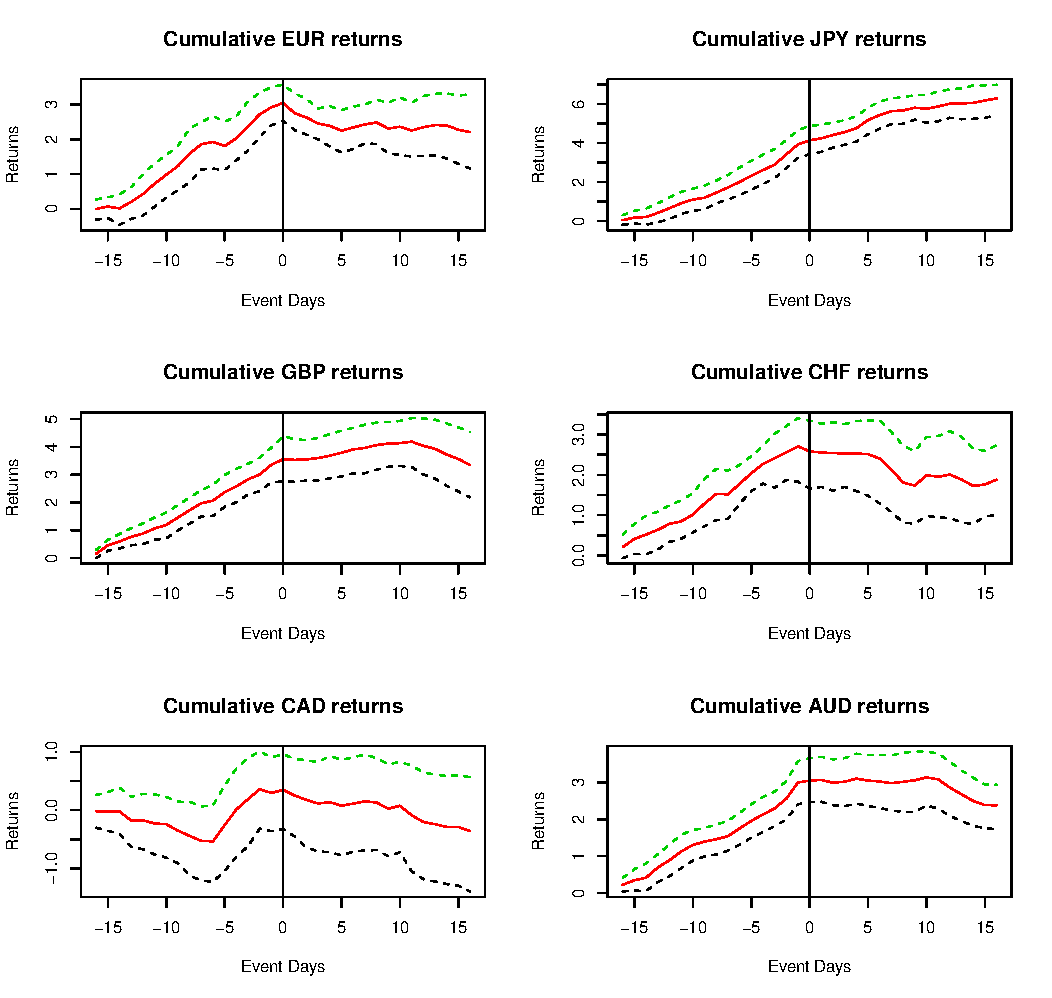
\includegraphics[scale=0.8]{RRCum16}
\caption{Event Study: Extreme (High $99{th}$ percentile) Risk Reversal Skew and 16 day event window: Risk reversals are the ratio of implied volatility on calls to the equivalent put; extreme high is at or above the $99^{th}$ percentile for the whole range, cumulative returns are the sum of log exchange rate returns. The event day is the day of the extreme risk reversal reading.  If speculation is uninformed, extremes should be followed by reversals; if speculation is informed, extremes are more likely to be followed by a random walk. The solid line is the cumulative mean return from the start of the event window; the dashed lines show the 95\% confidence intervals constructed from 1000 random bootstrap samples of appropriate event window day.}
\label{fig:ES5}
\end{figure}

\begin{figure}
\graphicspath{{../Figures/}}
\centering
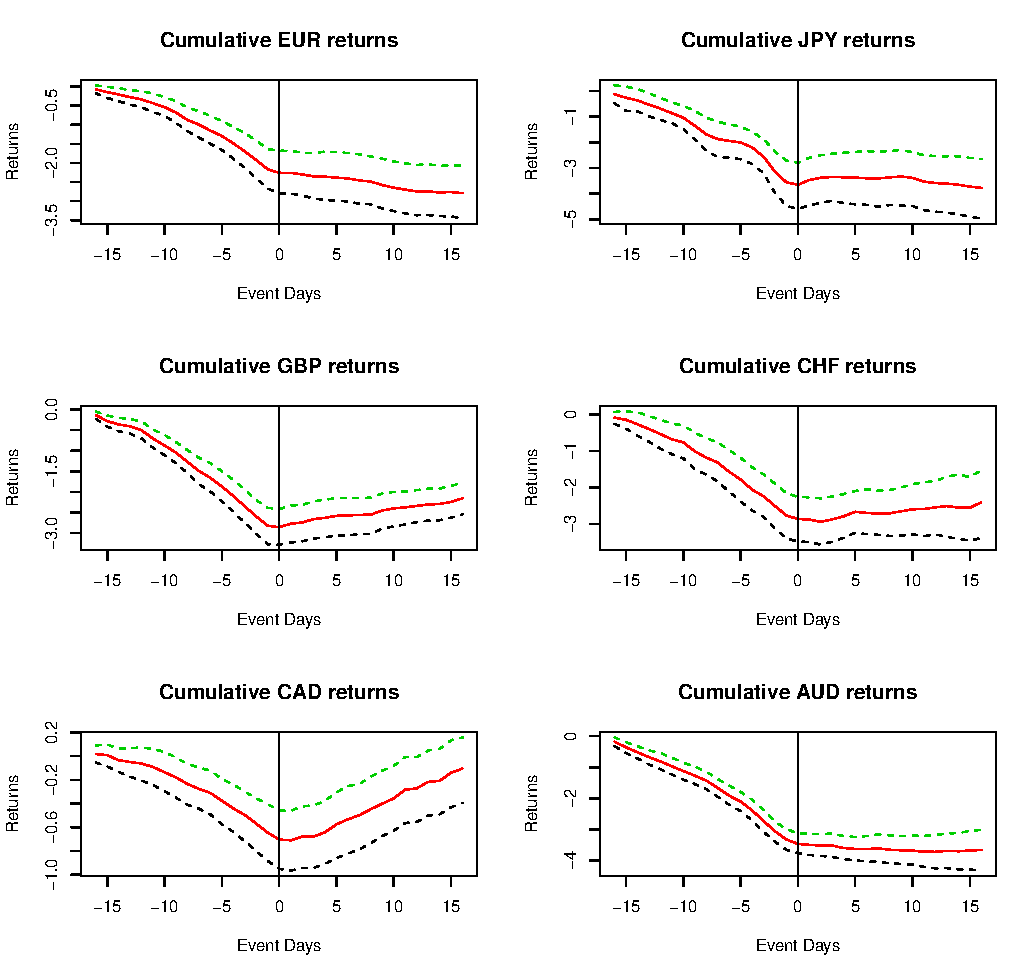
\includegraphics[scale=0.8]{RRCum16a}
\caption{Event Study: Extreme (Low $10{th}$ percentile) Risk Reversal Skew and 16 day event window: Risk reversals are the ratio of implied volatility on calls to the equivalent put; extreme low is at or below the $10^{th}$ percentile for the whole range, cumulative returns are the sum of log exchange rate returns. The event day is the day of the extreme risk reversal reading.  If speculation is uninformed, extremes should be followed by reversals; if speculation is informed, extremes are more likely to be followed by a random walk. The solid line is the cumulative mean return from the start of the event window; the dashed lines show the 95\% confidence intervals constructed from 1000 random bootstrap samples of appropriate event window day.}
\label{fig:ES2}
\end{figure}

\begin{figure}
\graphicspath{{../Figures/}}
\centering
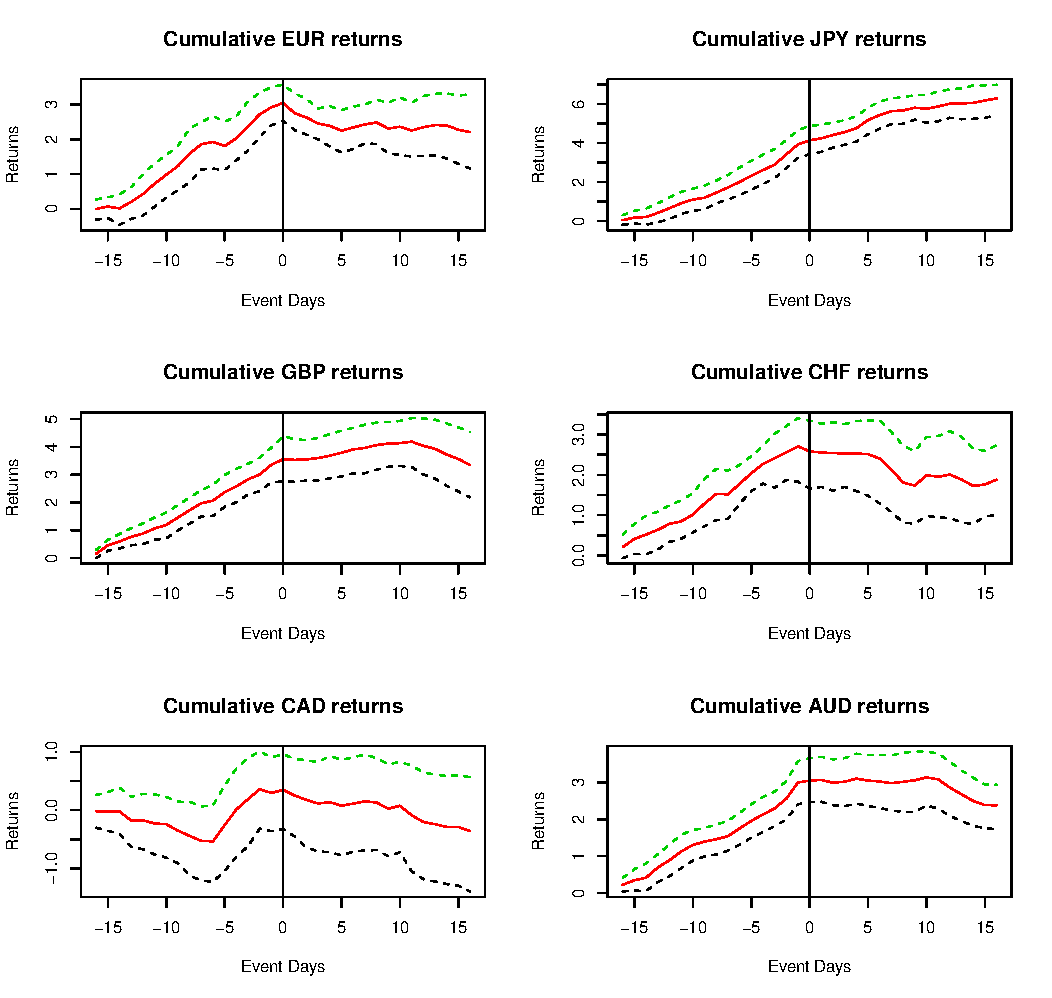
\includegraphics[scale=0.8]{RRCum16}
\caption{Event Study: Extreme (High $99{th}$ percentile) Risk Reversal Skew and 16 day event window: Risk reversals are the ratio of implied volatility on calls to the equivalent put; extreme high is at or above the $99^{th}$ percentile for the whole range, cumulative returns are the sum of log exchange rate returns. The event day is the day of the extreme risk reversal reading.  If speculation is uninformed, extremes should be followed by reversals; if speculation is informed, extremes are more likely to be followed by a random walk. The solid line is the cumulative mean return from the start of the event window; the dashed lines show the 95\% confidence intervals constructed from 1000 random bootstrap samples of appropriate event window day.}
\label{fig:ES1}
\end{figure}
 
Table \ref{tabref:SP1} shows the results from the event studies that were carried out using speculative positions as reported to US regulators.  The table works in a similar way to Table \ref{tabref:RR1}.  The first column is the exchange rate, defined as units per US dollar.  The table is then split into two parts.  The first part uses the S1 measure, the net non-commercial (speculative) positions relative to total non-commercial (speculative) positions; the second is S2 as the net non-commercial position relative to open interest or the total outstanding open positions.  Therefore, the first captures the balance of speculative positions while the second captures the balance of speculative positions relative to the whole market.  If speculators become more prevalent or dominant in the market, this will show up in S2 but not S1.  S1 is more sensitive to changes in sentiment and more volatile. Each of these sections is broken into the results for a 2 week window and a 4 week window.  There is a row for extreme high and extreme low which represents extreme long positions or extreme short positions; the first  column identifies the number of cases; CARW is the cumulative abnormal return for the whole event window; CARA is the cumulative abnormal return for the period after the event to the end of the window.     

\begin{sidewaystable}
% multirow package is required.   
%pdflandscape is required to facilitate the landscape position. 
\begin{threeparttable}
\caption{Event Study: Cumulative Abnormal Returns and Extreme Speculative Positions}
\begin{tabular}{llccccccccccccc}	
 % \hline
& &\multicolumn{6}{c}{S1 - Net Long per Speculators} & \multicolumn{1}{c}{} & \multicolumn{6}{c}{S2 -Net Long per Open Positions}\\
 & &\multicolumn{3}{c}{2 week} & \multicolumn{3}{c}{4 week} & \multicolumn{1}{c}{} & \multicolumn{3}{c}{2 week} & \multicolumn{3}{c}{4 week} \\ 
%\cline{4 - 10} \cline{13 - 19}
& &\multicolumn{1}{ c}{N} & \multicolumn{1}{c}{CARW} & \multicolumn{1}{c}{CARA} & \multicolumn{1}{ c}{N} & \multicolumn{1}{c}{CARW} & \multicolumn{1}{c}{CARA} & \multicolumn{1}{c}{} & 
\multicolumn{1}{ c}{N} & \multicolumn{1}{c}{CARW} & \multicolumn{1}{c}{CARA}  
& \multicolumn{1}{ c}{N} & \multicolumn{1}{c}{CARW} & \multicolumn{1}{c}{CARA}  \\   
\hline
\multirow{2}{*}{EUR} 
& Hi &  27 &  2.9415* & 1.3163* &27 & 3.8059* & 1.7341* &&27 & 1.0974* & 0.2896 &27 & 1.7667*& 0.0419  \\ 
& Lo & 27 & -2.4258* & -1.2512* & 27 &-3.9235* &-1.9254* & & 27 & -2.5122* & -1.0607* & 27 & -4.4478* & -1.9285* \\
\multirow{2}{*}{JPY}
& Hi & 43 & 1.9749* & 0.7286* & 43 & 2.8628* & 0.7909 & & 43 & 2.2463* & 1.0554* &43 & 3.7125* & 1.4443*  \\ 
& Lo & 43 & -2.2014* & -1.1312* & 43&-3.2488* & -1.5758* & &43 & -2.0605* & -0.9791* &43  & -2.6865* & -0.8318  \\
\multirow{2}{*}{GBP}
& Hi & 43 & 0.7102 & -0.2116 &43 & 1.0172* & -0.7902* & &43 & 1.2916* & 0.2370 &43 &1.6912* &0.0126  \\ 
& Lo & 43 &-0.6979* &0.2902 &43 &-1.5330* &0.1014 & &43 &-1.8993* &-0.1415 &43 &-2.8830* & -0.0768 \\
\multirow{2}{*}{CHF}
& Hi & 43 & 1.4400* & -0.0988 & 43 & 2.8665* & -0.0993 & & 43 &  2.5260* &  0.5074 & 43 & 3.6060* & 0.2158  \\ 
& Lo & 43 & -2.1816* &  -0.9770* & 43 &-3.3030* & -0.09798* & & 43 & -1.2605* & -0.3070& 43 &-0.1.6021* & 0.0670  \\
\multirow{2}{*}{CAD}
& Hi & 43 & 1.8658* & 1.0195* & 43 & 3.5298* & 1.8319* & & 43 & 2.0160* & 0.8788* &43 & 3.0995* & 0.9921*  \\ 
& Lo & 43 &-1.3238* & -0.5548* & 43 & -1.9151* & -0.7859* & & 43 & -1.2462* & -0.4505*  &43 & -1.9390*  & -0.6195*  \\
\hline
\label{tabref:SP1}
\end{tabular}
\begin{tablenotes}
\small 
\item Where Hi means extreme high, either S1 which is the measure of net long non-commercial (speculative) positions per total of speculators) or S2 which is the measure of net long non-commercial (speculative) positions per open interest (total outstanding open positions); high and low are above the $95^{th}$ percentile or below the $5^{th}$ percentile respectively; CARW is the cumulative abnormal return for the whole window, before and after the extreme event, and CARA is the cumulative abnormal return for the period after the event, which is the event day and the window; abnormal return is anything that is different from zero; the asterisk denotes significantly different from zero, where statistical significance is that more than 95\% of 1000 means calculated from random bootstraps from the extreme readings are above or below zero.   
\end{tablenotes}	
\end{threeparttable}  
\end{sidewaystable}

Once again, there is a very strong association between returns and the activity of speculators.  For the 4-day window and the S1 and S2 measures, every one of the currencies studied, high and low, had a mean cumulative return for the whole of the event window that was in the same direction as sentiment.  When re-sampled a thousand times, more than ninety five percent of the means calculated were greater than zero in all cases but one (GBP).  There is evidence here of momentum and of prices following the movement of speculator positions. 

\begin{figure}
\graphicspath{{../Figures/}}
\centering
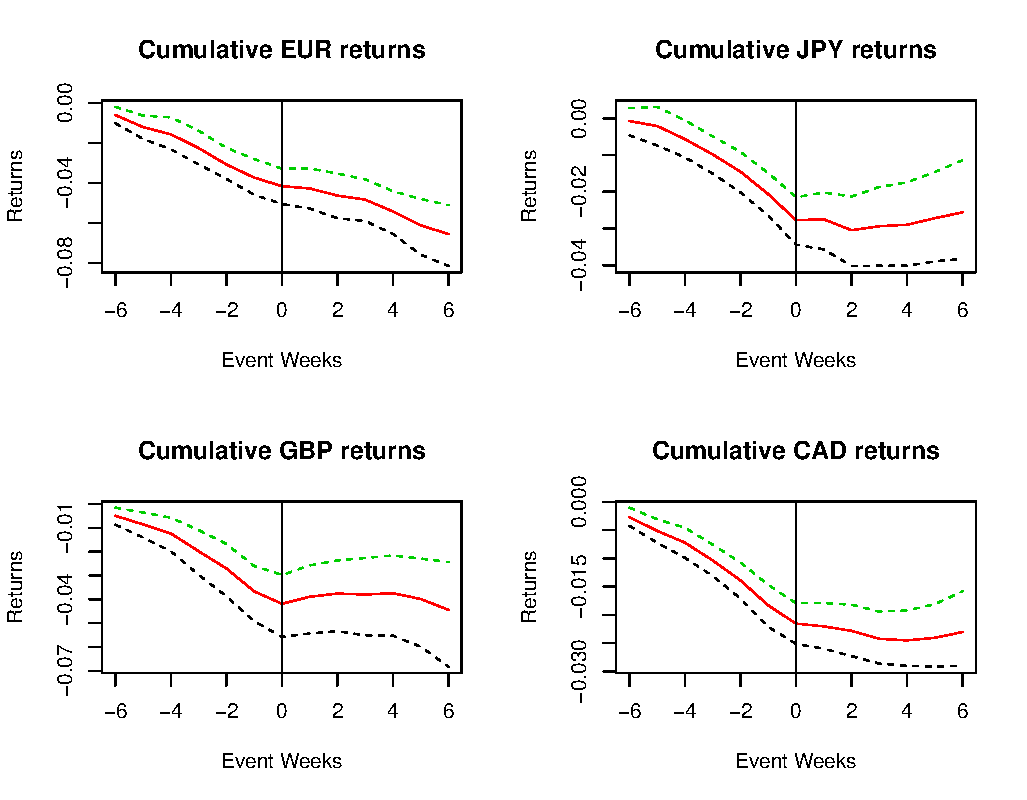
\includegraphics[scale=0.8]{FPCum6w}
\caption{Event Study: Extreme (Low $5{th}$ percentile) Risk Reversal Skew and 16 day event window: Risk reversals are the ratio of implied volatility on calls to the equivalent put; extreme low is at or above the $5^{th}$ percentile for the whole range, cumulative returns are the sum of log exchange rate returns. The event day is the day of the extreme risk reversal reading.  If speculation is uninformed, extremes should be followed by reversals; if speculation is informed, extremes are more likely to be followed by a random walk. The solid line is the cumulative mean return from the start of the event window; the dashed lines show the 95\% confidence intervals constructed from 1000 random bootstrap samples of appropriate event window day.}
\label{fig:ES3}
\end{figure}

\begin{figure}
\graphicspath{{../Figures/}}
\centering
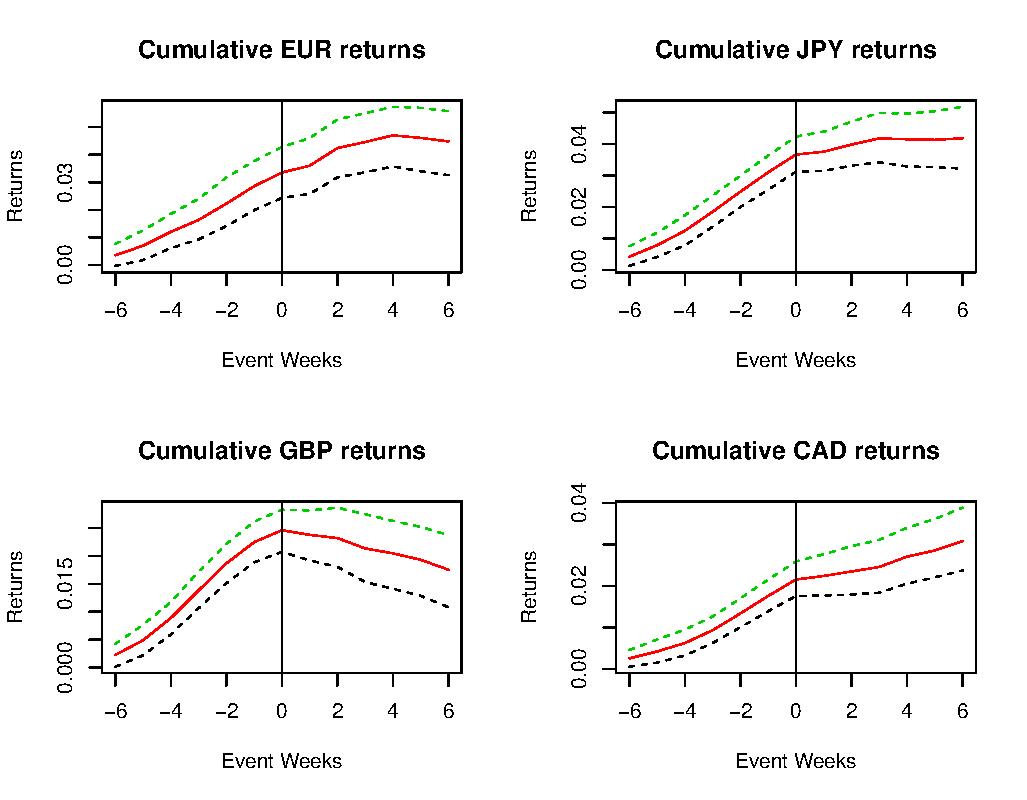
\includegraphics[scale=0.8]{FPCum6wa}
\caption{Event Study:  Extreme ($90^{th}$ percentile), Non-commercial net long (S1), 6 week window. Non-commercial net per OI (S2) are the net speculative positions (as reported to US regulator the CFTC) relative to all open positions; extreme high is at or above the $90^{th}$ percentile for the whole range, cumulative returns are the sum of log exchange rate returns. The event day is the day of the extreme reading as a measure of extreme speculative activity.  If speculation is uninformed, extremes should be followed by reversals; if speculation is informed, extremes are more likely to be followed by a random walk.}
\label{fig:ES4}
\end{figure}

There is little evidence that these self-reported speculators are driving prices away from fundamentals with their activity. Sixty percent of the S1 cases still show a significant abnormal return in the direction of the extreme 4 weeks after the extreme has been reached; only thirty percent of the cases show a reversal and in only one of those do ninety five percent of the means calculated after re-sampling remain above zero.  For S2 there is even less clarity, with ninety percent of the cases showing a continuation and forty percent of them showing significant continuation.  The evidence here with speculative positions is the same as that of speculative sentiment.  Prices move in the direction of speculative activity but speculative extremes do not provide information about the future. The price action of the event study is consistent with speculation being informed rather than uninformed.     

\section{Speculation and foreign exchange returns}
If foreign exchange speculation is uninformed noise, extreme speculation, whether measured by sentiment or weight of activity, will coincide with deviations from fundamental value; if speculation is informed, speculation is part of the process of price discovery and extremes will provide no information and future prices will follow a random walk. An event study showed that speculation is associated with price movement: exchange rates move in the direction of speculative sentiment and activity.  However, once extreme, prices are as likely to continue as to reverse.  

The results that are recorded are not a function of the design of the event study.  The event window and the quantile that is chosen to measure the extreme can be changed.  Alternative measures produced very similar results. Alternative quantiles from 1\% and 99\% to 20\% and 80\% have also been assessed.  Figures \ref{fig:ES1}, \ref{fig:ES2}, \ref{fig:ES3} and \ref{fig:ES4} have much wider windows and do not find any alternative to the view that extreme speculation is followed by a random walk. 

The covariance of speculative sentiment and speculative positions with the return indicates that this activity influences prices.  It is not random.  These results show that foreign exchange speculation, whether measured using either sentiment or the weight of positions, is an important part of the price discovery process.  The random walk after the extreme is indicative of foreign exchange prices absorbing most of the information that is available.  

It is encouraging that these two very different measures of speculative activity produce very similar results and that the results hold over different time frames: one week for the option data and one week for the regulatory position data.  It is less clear whether the results would be reproduced across markets for other financial assets.    These results do not rule out uninformed speculation.  The Friedman effect from the Noise-trader model depends on there being \emph{noise-trader risk} or some limits to arbitrage.  The effect is not evident in this study of foreign exchange.  However, this is a large and very liquid market, other asset classes may have alternative institutional features that many not mean that these results can be extrapolated without important institutional questons being asked.

The \emph{Tobin Tax} would put a charge against financial transactions, particularly in foreign exchange.  Part of the argument depends on speculation being uninformed as the reduced activity that is caused by the tax would, it is argued, limit volatility and allow more long-term fundamental evaluations to become more prominent.  However, if speculation is informed and part of the price discovery process, this tax may reduce liquidity and increase volatility. 

\bibliography{../../myrefs}

\end{document}

